\documentclass[border=10pt]{standalone}
\usepackage{tikz}
\usepackage{amsmath}
\usetikzlibrary{arrows.meta}

\begin{document}
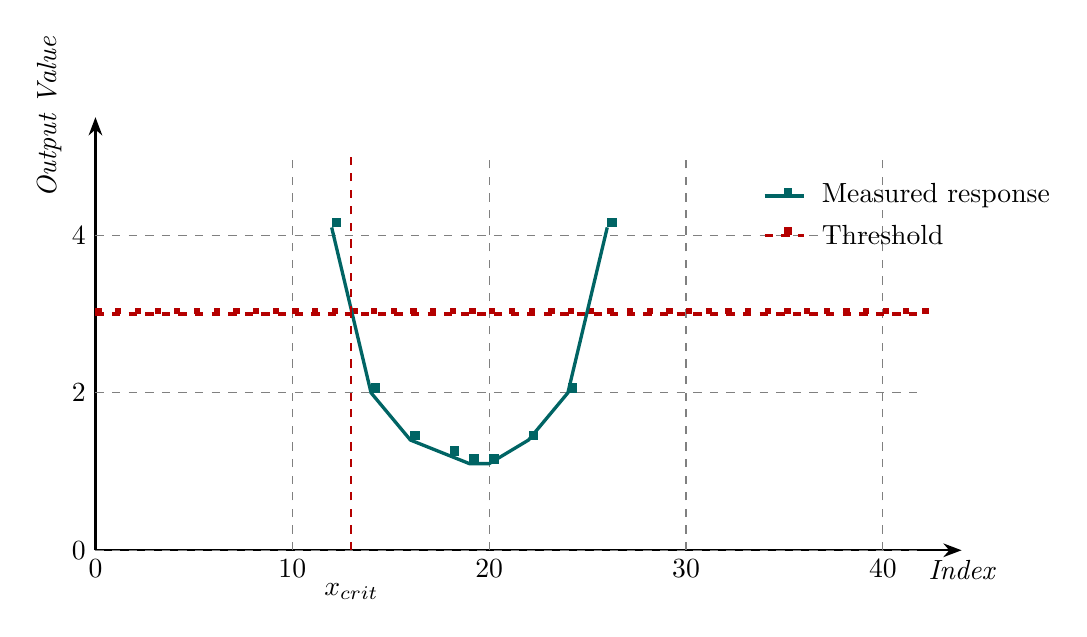
\begin{tikzpicture}[>=Stealth]
    % Define colors
    \definecolor{tealcolor}{RGB}{0,100,100}
    \definecolor{redcolor}{RGB}{180,0,0}
    
    % Axis
    \draw[thick, ->] (0,0) -- (11,0) node[below, font=\itshape] {Index};
    \draw[thick, ->] (0,0) -- (0,5.5) node[above, rotate=90, anchor=south, font=\itshape, yshift=0.3cm] {Output Value};
    
    % Grid
    \foreach \x in {0,2,4} {
        \draw[gray, dashed] (0,\x) -- (10.5,\x);
    }
    \foreach \x in {2.5,5,7.5,10} {
        \draw[gray, dashed] (\x,0) -- (\x,5);
    }
    
    % Y-axis labels
    \foreach \y in {0,2,4} {
        \node[left] at (0,\y) {\y};
    }
    
    % X-axis labels
    \foreach \x/\label in {0/0,2.5/10,5/20,7.5/30,10/40} {
        \node[below] at (\x,0) {\label};
    }
    
    % Threshold line
    \draw[redcolor, thick, dashed, line width=1.2pt] 
        (0,3) -- (10.5,3);
    
    % Threshold markers
    \foreach \x in {0,0.25,...,10.5} {
        \fill[redcolor] (\x,3) rectangle ++(0.08,0.08) ++(-0.04,-0.04);
    }
    
    % Measured response data
    \coordinate (p1) at (3,4.1);
    \coordinate (p2) at (3.5,2);
    \coordinate (p3) at (4,1.4);
    \coordinate (p4) at (4.5,1.2);
    \coordinate (p5) at (4.75,1.1);
    \coordinate (p6) at (5,1.1);
    \coordinate (p7) at (5.5,1.4);
    \coordinate (p8) at (6,2);
    \coordinate (p9) at (6.5,4.1);
    
    % Draw measured response line
    \draw[tealcolor, thick, line width=1.2pt] 
        (p1) -- (p2) -- (p3) -- (p4) -- (p5) -- (p6) -- (p7) -- (p8) -- (p9);
    
    % Measured response markers
    \foreach \p in {p1,p2,p3,p4,p5,p6,p7,p8,p9} {
        \fill[tealcolor] (\p) rectangle ++(0.12,0.12) ++(-0.06,-0.06);
    }
    
    % Critical point line
    \draw[redcolor, thick, dashed] (3.25,0) -- (3.25,3);
    \draw[redcolor, thick, dashed] (3.25,3) -- (3.25,5);
    
    % x_crit label
    \node[below, font=\itshape] at (3.25,-0.3) {$x_{crit}$};
    
    % Legend
    \begin{scope}[shift={(8.5,4.5)}]
        % Measured response
        \draw[tealcolor, thick, line width=1.2pt] (0,0) -- (0.5,0);
        \fill[tealcolor] (0.25,0) rectangle ++(0.1,0.1) ++(-0.05,-0.05);
        \node[right, font=\rmfamily] at (0.6,0) {Measured response};
        
        % Threshold
        \draw[redcolor, thick, dashed, line width=1.2pt] (0,-0.5) -- (0.5,-0.5);
        \fill[redcolor] (0.25,-0.5) rectangle ++(0.1,0.1) ++(-0.05,-0.05);
        \node[right, font=\rmfamily] at (0.6,-0.5) {Threshold};
    \end{scope}
    
\end{tikzpicture}
\end{document}